In this section, we empirically evaluate STOIC's performance on executing machine learning applications, in contrast to single-runtime systems. We first outline the machine learning application benchmark that we consider, followed by our test on the application efficacy. Then an empirical experiment and its results are presented.

\subsection{Benchmark Application and Dataset}

We benchmark STOIC using an image processing application that classifies animal images from a wildlife monitoring system called ``Where's The Bear" (WTB)~\cite{ref:wtb}. ``Where's The Bear" is an end-to-end distributed data acquisition and analytics system that implements an IoT architecture and edge cloud. Our application inferences streaming photos taken by wildly deployed camera traps in Sedgwick Natural Reserve using a convolutional neural network (CNN)~\cite{ref:cnn} model trained by labeled images from the WTB dataset. Technically, it employs Tensorflow and Scikit-learn~\cite{ref:scikit} machine learning frameworks to perform the image classification.  

 In total, there are five classes that we consider in the CNN model training: Bird, Fox, Rodent, Human and Empty. Since the volume of classes are unbalanced due to different occurring frequency of animals, we up-sample the minority classes (e.g. fox) by Keras ImageDataGenerator~\cite{ref:keras} to ensure the classification model is not biased. We resize every image in the WTB dataset to $1920 \times 1080$, and for each class, the dataset contains 251 images used to train the CNN model. Once the model is trained, the application caches this model in hdf5 format and store it at both edge cloud disk storage and a shared volume in the Ceph file system at Nautilus cloud. 

\subsection{Application Efficacy}

\begin{table}[t] \centering 
\scriptsize
\resizebox{\columnwidth}{!}{
\begin{tabular}{|c|c|c|c|c|} 
\hline
& \textbf{Mean $T_r$ (sec)} & \textbf{Stdev. $T_r$ (sec)} & \textbf{Mean $T_p$ (sec)} & \textbf{Stdev. $T_p$ (sec)}\\
\hline
edge & 108.88 & 1.65 & 108.88 & 1.65 \\
\hline
cpu & 100.0 & 4.93 & 86.99 & 4.92 \\
\hline
gpu1 & 98.90 & 4.03 & 50.65 & 4.05 \\
\hline
gpu2 & 106.29 & 5.53 & 39.21 & 5.55\\
\hline
\textbf{STOIC} & \textbf{97.73} & \textbf{3.13} & \textbf{50.49} & \textbf{3.11} \\
\hline
\end{tabular}
}
\caption{\textbf{Mean and stdev of total response time~($T_r$) and processing time~($T_p$) of 40-image batch}: STOIC schedules tasks onto the runtime (\textit{gpu1}) that has the least total response time~($T_r$).
\label{tab:validation}}
\end{table}

We first test the efficacy of STOIC by processing an image batch of fixed size at four runtimes individually and then compare them with STOIC. To make the result reliable, we again conduct the experiment 10 times and list the mean and standard deviation of total response time~($T_r$) and processing time~($T_p$) in Table~\ref{tab:validation}. We can observe from Table~\ref{tab:validation} that STOIC schedules 40-image batch to \textit{gpu1} runtime, based on its prediction that  \textit{gpu1} would have the least total response time~($T_r$). One important observation is that \textit{gpu2} runtime has even lower processing time~($T_p$) than \textit{gpu1}, but STOIC disregard \textit{gpu2} in this scenario, because its gain in processing time~($T_p$) does not compensate for its lengthy deployment time~($T_d$) on Nautilus cloud.

\begin{figure}[t] \centering 
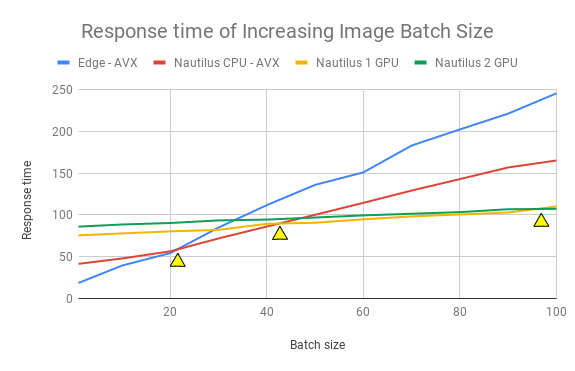
\includegraphics[scale=0.32]{response-time}
\caption{\textbf{Total Response Time~($T_r$) of image batches of growing sizes}: The x-axis represents the batch size, while the y-axis is the total response time~($T_r$). STOIC, which is depicted in the blue dashed line, schedules the task on the runtime with the least total response time.  
\label{fig:response-time}}
\end{figure}

Additionally, we test STOIC by processing a series of image batches of growing sizes both on four runtimes and STOIC. The progressive response times are depicted in Figure~\ref{fig:response-time}. The x-axis is the size of the image batch and the y-axis is the total response time~($T_r$) in seconds. The red curve represents the linearly increasing latency from \textit{edge} runtime, whereas the yellow one depicts that for \textit{cpu} runtime at Nautilus cloud. We observe that its slope is more moderate than \textit{edge} runtime since CPUs in nodes of Nautilus cloud are usually more powerful than edge cloud. The pink and green curve represent the \textit{gpu1} and \textit{gpu2} runtime respectively and they intersect at the batch size of 95, at which STOIC would switch the deployment of task from \textit{gpu1} to \textit{gpu2}. The blue dashed line depicts the total response time~($T_r$) of STOIC, which is able to schedule a series of tasks to the runtime with the least latency. According to such a result, we ensure STOIC improves system performance by dynamic scheduling based on image batch size.


\subsection{Empirical Experiment}


% \begin{table}[t]
%     \centering
%     \scriptsize

\begin{tabular}{|c|c|c|c|c|c|} 
\hline
\textbf{Runtimes}& \textbf{edge} & \textbf{cpu} & \textbf{gpu1} & \textbf{gpu2} & \textbf{STOIC} \\
\hline
Avg. $T_r$ (sec) & 2842.58 & 2065.59 & 2173.98 & 2201.02 & 1931.64 \\
\hline
Speed-up (\%) & 32.05 & 6.48 & 11.15 & 12.24 & N/A \\
\hline
\end{tabular}

%     \caption{\textbf{Average total response time~($T_r$) and speed-up on 24-hour dataset}: Comparing with four single runtimes, STOIC achieves lowest average latency and speed-up ranging from 6.48\% to 32.05\%. }
%     \label{tab:24-batches}
% \end{table}


As an empirical evaluation of STOIC, we compare the total response time~($T_r$) of multiple image batches of varying sizes by four single runtimes and STOIC. To accelerate the repetitive experiment, we developed a simulator to generate image batches based on the frequency distribution of the WTB dataset. According to 2016 WTB dataset, the size of image batch fits to normal distribution $\mathbf{N}(\mu = 42.75, \sigma^2 = 39.5)$. Thus, the simulator generates 24 image batches in the edge controller to emulate streaming data in one day from open field camera traps. To conduct an unbiased evaluation, we seed the simulator to make these 24 image batches consistent across all runtimes and STOIC. 

\begin{figure}[t] \centering 
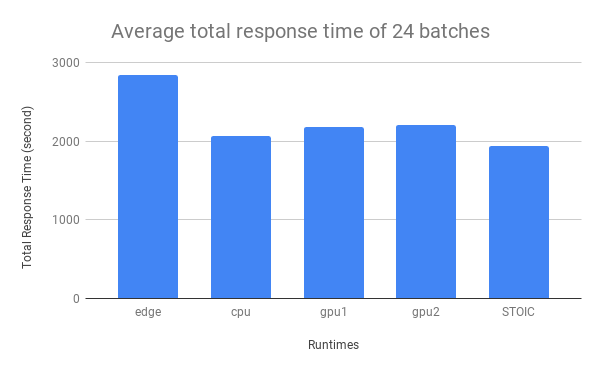
\includegraphics[scale=0.42]{figures/24-batches}
\caption{\textbf{Avg. total response time~($T_r$) on the 24-hour dataset}: The x-axis represents runtimes, while the y-axis represents the average total response time~($T_r$) by STOIC and four other runtimes on the 24-hour dataset. The data labels on columns are specific numbers of $T_r$. The 24-hour batch sizes are generated from the distribution of historical data. 
\label{fig:24-batch}}
\end{figure}

To ensure the validity of outcome, We again run such an experiment 10 times for each runtime scenario and report the average value. Figure~\ref{fig:24-batch} demonstrates the average total response time~($T_r$) for STOIC and four individual runtimes. Specifically, STOIC achieves the lowest average latency among four other single runtimes and reduces total response time~($T_r$) by 32.05\% (\textit{edge}), 6.48\% (\textit{cpu}), 11.15\% (\textit{gpu1}) and 12.24\% (\textit{gpu2}) respectively. According to such a result, we conclude that STOIC outperforms single-runtime scheduling mechanism on the empirical datasets and real-world machine learning applications.
